\subsection{Client mobile et serveur}
Le client mobile s'occupe de la connexion au serveur et de lancer le jeu.
Une première activité lui permet de saisir l'adresse du serveur et son nom d'utilisateur, elle permet aussi d'afficher les messages d'erreur de connexion. Une seconde activité affiche une liste d'utilisateurs connectés, autrement dit le \textit{lobby} ou \textit{salon} de la partie, ainsi que deux boutons \verb!ready! et \verb!leave!.

\begin{figure}
\begin{center}
\fbox{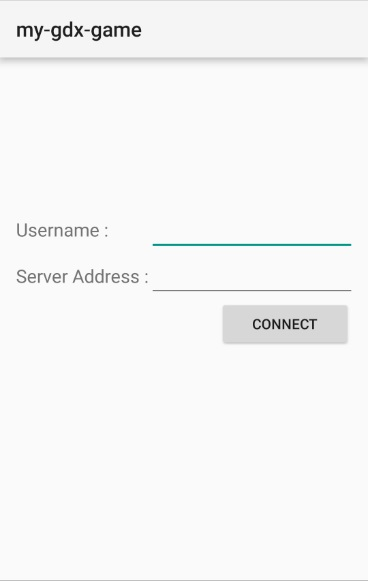
\includegraphics[scale=0.5]{images/jeu1.jpg}}
\end{center}
\caption{Connexion}
\end{figure}

\begin{figure}
\begin{center}
\fbox{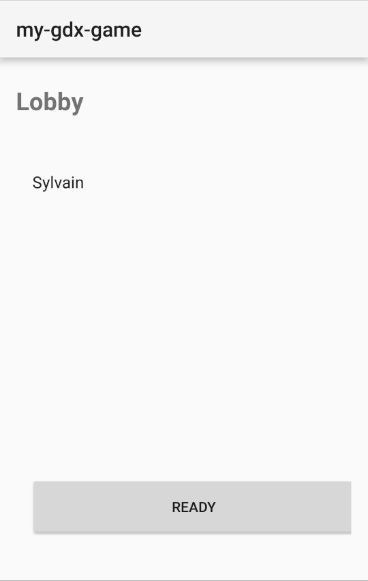
\includegraphics[scale=0.5]{images/jeu2.jpg}}
\end{center}
\caption{Lobby}
\end{figure}

Le serveur s'occupe d'une partie : il commence par attendre que les joueurs se connectent sur le lobby de la partie. Lorsque tout les joueurs ont signalé qu'ils sont prêts, il lance la partie et notifie à tout les clients de lancer le jeu.

Un seul niveau prédéfini de longueur fixe est disponible pour le moment. Lorsque les joueurs atteignent un objectif, en le touchant au bon moment, leur client envoie un message indiquant le score qu'ils ont obtenu. Le serveur met donc à jour le score des différents joueurs et, lorsque le temps imparti est écoulé, notifie les clients que la partie est terminée et leur indique le gagnant.

Pour implémenter ces communications nous avons utilisé le protocole \verb!UDP!. Une difficulté rencontrée sur cette partie fût que le message permettant au serveur de notifier le client que sa connexion est acceptée et de lui octroyer son numéro de communication (permettant d'identifier le client à l'origine du message reçu), n'était pas reçu dans 100 \% des cas. Plusieurs séances de tests ne posèrent aucuns problèmes tandis que, d'autres fois, la connexion échouait côté client, laissant un \og client fantôme \fg{} sur le serveur.

L'origine de ce problème n'a pas pu être identifié à ce jour et n'est remarqué que sur des communications entre des appareils android et un ordinateur.
Il peut être corrigé en passant par des communications \verb!TCP! qui sont protégées contre la perte de paquets et les erreurs de transmission, permettant ainsi de s'abstraire de l'identifiant des clients, car les communications côté serveur dans ce cas seraient distribuées sur plusieurs \textit{socket}.
